\section{Motivation and High Level Considerations}

The most straightforward way of improving the performance of deep neural networks is by increasing their size. This includes both increasing the depth -- the number of levels -- of the network and its width: the number of units at each level. This is as an easy and safe way of training higher quality models, especially given the availability of a large amount of labeled training data. However this simple solution comes with two major drawbacks. 

Bigger size typically means a larger number of parameters, which makes the enlarged network more prone to overfitting, especially if the number of labeled examples in the training set is limited. This can become a major bottleneck, since the creation of high quality training sets can be tricky and expensive, especially if expert human raters are necessary to distinguish between fine-grained visual categories like those in ImageNet (even in the 1000-class ILSVRC subset) as demonstrated by Figure~\ref{fig:finegrained}.

\begin{figure}
\centering
\subfigure[Siberian husky]{
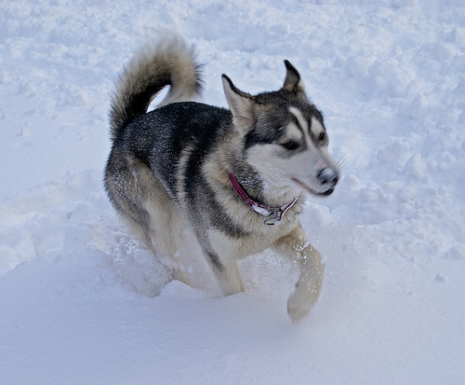
\includegraphics[width=0.49\textwidth]{siberianhusky.pdf}
\label{fig:siberianhusky}
}
\subfigure[Eskimo dog]{
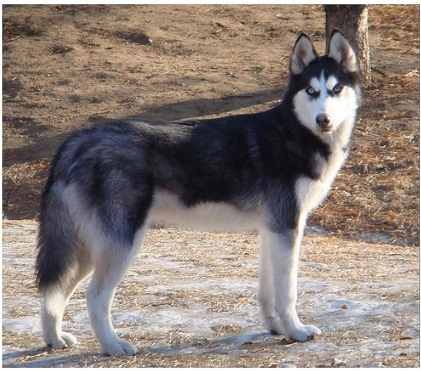
\includegraphics[width=0.4658\textwidth]{Eskimodog.pdf}
\label{fig:eskimodog}
}
\caption{Two distinct classes from the 1000 classes of the ILSVRC 2014 classification challenge.}
\label{fig:finegrained}
\end{figure}

Another drawback of uniformly increased network size is the dramatically increased use of computational resources. For example, in a deep vision network, if two convolutional layers are chained, any uniform increase in the number of their filters results in a quadratic increase of computation. If the added capacity is used inefficiently (for example, if most weights end up to be close to zero), then a lot of computation is wasted. Since in practice the computational budget is always finite, an efficient distribution of computing resources is preferred to an indiscriminate increase of size, even when the main objective is to increase the quality of results.

The fundamental way of solving both issues would be by ultimately moving from fully connected to sparsely connected architectures, even inside the convolutions. Besides mimicking biological systems, this would also have the advantage of firmer theoretical underpinnings due to the groundbreaking work of Arora et al.~\cite{arora2013bounds}. Their main result states that if the probability distribution of the data-set is representable by a large, very sparse deep neural network, then the optimal network topology can be constructed layer by layer by analyzing the correlation statistics of the activations of the last layer and clustering neurons with highly correlated outputs. Although the strict mathematical proof requires very strong conditions, the fact that this statement resonates with the well known Hebbian principle -- neurons that fire together, wire together -- suggests that the underlying idea is applicable even under less strict conditions, in practice.

On the downside, today’s computing infrastructures are very inefficient when it comes to numerical calculation on non-uniform sparse data structures. Even if the number of arithmetic operations is reduced by $100{\times}$, the overhead of lookups and cache misses is so dominant that switching to sparse matrices would not pay off. The gap is widened even further by the use of steadily improving, highly tuned, numerical libraries that allow for extremely fast dense matrix multiplication, exploiting the minute details of the underlying CPU or GPU hardware~\cite{song2014scaling, krizhevsky2012imagenet}. Also, non-uniform sparse models require more sophisticated engineering and computing infrastructure. Most current vision oriented machine learning systems utilize sparsity in the spatial domain just by the virtue of employing convolutions. However, convolutions are implemented as collections of dense connections to the patches in the earlier layer. ConvNets have traditionally used random and sparse connection tables in the feature dimensions since~\cite{lecun1998gradient} in order to break the symmetry and improve learning, the trend changed back to full connections with \cite{krizhevsky2012imagenet} in order to better optimize parallel computing. The uniformity of the structure and a large number of filters and greater batch size allow for utilizing efficient dense computation.

This raises the question whether there is any hope for a next, intermediate step: an architecture that makes use of the extra sparsity, even at filter level, as suggested by the theory, but exploits our current hardware by utilizing computations on dense matrices. The vast literature on sparse matrix computations (e.g.~\cite{catalyurek2010sparse}) suggests that clustering sparse matrices into relatively dense submatrices tends to give state of the art practical performance for sparse matrix multiplication. It does not seem far-fetched to think that similar methods would be utilized for the automated construction of non-uniform deep-learning architectures in the near future.

The Inception architecture started out as a case study of the first author for assessing the hypothetical output of a sophisticated network topology construction algorithm that tries to approximate a sparse structure implied by \cite{arora2013bounds} for vision networks and covering the hypothesized outcome by dense, readily available components. Despite being a highly speculative undertaking, only after two iterations on the exact choice of topology, we could already see modest gains against the reference architecture based on \cite{lin2013nin}. After further tuning of learning rate, hyperparameters and improved training methodology, we established that the resulting Inception architecture was especially useful in the context of localization and object detection as the base network for~\cite{girshick2014rich} and ~\cite{erhan2014scalable}. Interestingly, while most of the original architectural choices have been questioned and tested thoroughly, they turned out to be at least locally optimal.

One must be cautious though: although the proposed architecture has become a success for computer vision, it is still questionable whether its quality can be attributed to the guiding principles that have lead to its construction. Making sure would require much more thorough analysis and verification: for example, if automated tools based on the principles described below would find similar, but better topology for the vision networks. The most convincing proof would be if an automated system would create network topologies resulting in similar gains in other domains using the same algorithm but with very differently looking global architecture. At very least, the initial success of the Inception architecture yields firm motivation for exciting future work in this direction.
